\chapter{Introduction}
\label{chap:1}
\section{Motivation}

\newacronym{ai}{AI}{Artificial Intelligence}

\subsubsection*{Singularity Avoidance Control of VSCMG}
\newacronym{cmg}{CMG}{Control Moment Gyroscope}
\newacronym{vscmg}{VSCMG}{Variable Speed Control Moment Gyroscope}
Evident presence of singularities in \acrfull{cmg} and escaping them by adding an extra degree of freedom by using \acrfull{vscmg} to escape singular states is highly complex and nonlinear multi-input multi-output problem making it suitable choice to be evaluated on machine learning models. Moreover, a sub-optimal neural network approximation of nonlinear optimum function requires much less computing resources and memory storage than optimum guidance law\cite{Santoni1996}. Although machine learning based models are widely used in everyday applications ranging from image processing, weather prediction to Alpha Go being the first computer program to defeat human player in game of Go, \cite{Silver2016} their use in mission-critical task is limited.  This thesis is to evaluate the performance and technological readiness level of Neural Network based control model. 

\subsubsection*{The Test Bench}
It is difficult to evaluate the performance of the control law on real hardware and always been challenging to carry out hardware in the loop simulation of the attitude control system on the ground. Implementing complete 360 degrees of angular freedom of three body axes observed in orbit is indispensably difficult to attain inside ground-based laboratory. There has been a wide variety of technological solutions proposed and implemented since the beginning of the space age. Compromising with a reduced degree of freedom a platform balancing on sharp pin with its center of mass kept closer to pivot is chosen to keep the cost of the entire test setup as low as possible. 
Accessibility of 3D printing technology provides leverage for rapid prototyping of complex geometries. Goal behind hardware setup design is to provide an educational platform for preliminary evaluation and hardware in loop simulation of spacecraft attitude control system.

\vspace*{10px}
\begin{center}
\textit{``It doesn't matter how beautiful your theory is, it doesn't matter how smart you are. If it doesn't agree with experiment, it's wrong."} 
\flushright - Richard P. Feynman

\end{center}
\newacronym{acs}{ACS}{Attitude Control System}

\section{Literature Survey}
\acrfull{acs} being the primary subsystem of any spacecraft mission, based on the mission requirements a spacecraft must perform slew maneuvers for precise retargeting and maintaining desired state in presence of external disturbances. Important components of attitude determination and Control System are estimating the state of spacecraft using observations from sensors, actuators to provide required control torque towards reaching desired state and control algorithm to evaluate best inputs for actuators. Various types of actuators used in space missions each having its advantages and drawbacks over others. Typical examples are thrusters, magneto torquers, reaction wheels and control moment gyroscopes. Depending on mission requirements there are possible passive ways to maintain attitude of spacecrafts incorporating spin stabilization, solar sail, and gravity gradient. 
\begin{figure}[h!]
    \centering
    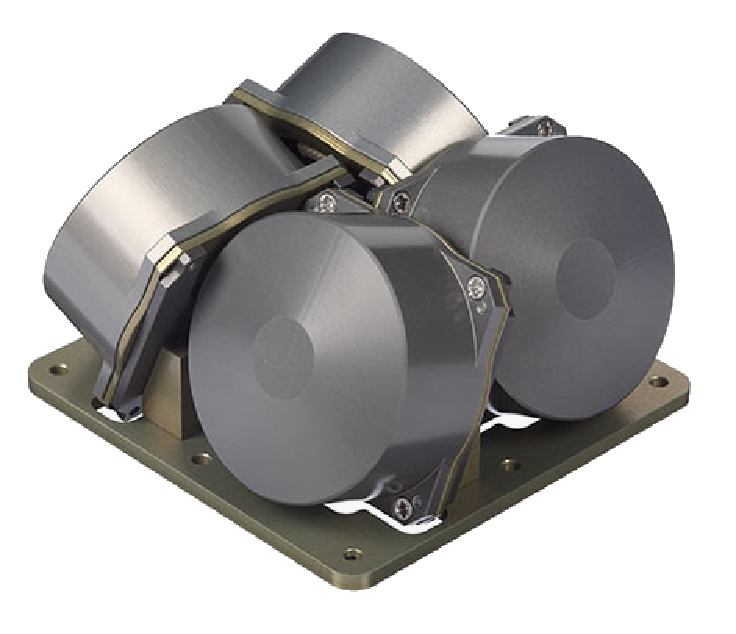
\includegraphics[width=0.5\linewidth]{figures/SatBus-4RW0-1-new.pdf}
    \caption{NanoAvionics (4RW0) integral four - reaction wheels redundant 3-axis control system  }
    \label{fig:na4RW0}
\end{figure}

\noindent Large spacecraft typically used in human spaceflight missions requires large and fast attitude maneuvers, this large demand torque requirement is generally achieved using reaction thrusters. Spacecrafts such as Apollo, Soyuz reentry vehicle used thruster-based \acrshort{acs}. Most recently SpaceX Dragon capsule is equipped with 16 DRACO thrusters \cite{web:SpaceXDargon} for orbit and attitude adjustment capable of producing 400N thrust each.\cite{book:SPACEX} Although being capable of producing large amount of control torques, mission life is limited by finite amount of fuel moreover exhaust fumes may have adverse effects on payload.
\newacronym{ladee}{LADEE}{Lunar Atmosphere and Dust Environment Explorer}
\newacronym{rw}{RW}{Reaction Wheel}
\newacronym{mw}{RW}{Reaction Wheel}
\newacronym{ipacs}{IPACS}{Integrated Power Attitude Control System}

For long duration missions having no possible means of refueling and high pointing accuracy requirements such as Hubble, Kepler Telescopes or optical communication demonstrator like \acrfull{ladee}, Momentum Exchange devices such as \acrfull{rw} or \acrfull{mw} are employed. Perhaps only difference is RWs are at rest at the beginning of mission, whereas MWs are spinning at maximum speed giving gyroscopic stiffness to spacecraft.
Reaction Wheels are used for \acrshort{acs}. Reaction Wheel is a momentum storage device consist of high inertia flywheel attached to an electric brush-less motor with its spin axis kept constant and aligned with spacecraft body. Torque is produced around axis of rotation by changing spin speed of flywheel, since total angular momentum of spacecraft must be conserved, spacecraft counter rotates proportionally to inertia ratio of body and reaction wheel. Very small and precise torques are produced by accelerating flywheels. Satellites are equipped with at least three reaction wheels are required to have complete attitude control capability some use four reaction wheels configuration for redundancy in case of failure as shown in Figure \ref{fig:na4RW0}. Excess energy produced by solar panels during exposure to sun can be stored in RW by means of momentum hence also known as mechanical batteries. Momentum Wheels can be used for both attitude control and mechanical batteries by incorporating \acrfull{ipacs}. \cite{TsiotrasPowerTracking} 

Apart from being very quick and precise internal torque production capabilities Reaction Wheels are limited by maximum angular momentum storage capacity and undergoes saturation. Inability to counteract disturbances on reaching maximum speed is major drawback and thus Reaction wheels must be used with other external torque-based actuators for de-saturation. For large satellites, thruster-based \acrshort{acs} is used for denaturation whereas small satellites often equipped with Magneto Torquers. Current passed through coil of electromagnet attached to spacecraft which creates magnetic dipole. Produced torque is vector product of ambient magnetic flux density vector and magnetic dipole of electromagnet.

Spinning mass has inherent tendency to maintain its axis of rotation. If spin axis is tilted a torque is observed transverse to spin and tilt axis this phenomenon is known as gyroscopic couple. A Control Moment Gyroscope is momentum exchange device consist of a flywheel and one or two motorized gimbles to tilt its spin axis. Flywheel spinning at high angular velocity, hence having high angular momentum. Large "torque amplification" caused by gyroscopic effect produced due to changing orientation of flywheel spin axis is vector cross product of angular momentum of flywheel and velocity of gimble axis rotation.\cite{Leve2015} CMGs are more power efficient than MWs since maintaining wheel spin requires small amount of power. CMGs are classified in two main categories based on number of degrees of freedom of RW spin axis. Single Gimble Control Moment Gyroscope (SGCMG) has one motorized gimble whereas Double Gimble Control Moment Gyroscope (DGCMG) incorporates two gimbles to tilt spin axis of flywheel. SGCMGs are more power efficient than DGCMG since to produce same amount of torque DGCMG requires more electric power. DGCMGs are heavier, requires complex electromechanical components to drive three nested motors. Only advantage of DGCMG is when momentum storage is primary requirement. As size of reaction wheel increased the complexity of DGCMG and its support mechanism keeps increasing due to extra gimble and it becomes no longer feasible. It is also important to avoid alinement of two axis to prevent gimble lock.\cite{ Markley2014} 

One of the earliest research related to use of control moment gyroscope as secondary actuator for gravity gradient stabilize satellite dates to 1964, CMG can act as both actuator and gyro sensor to sense vehicle rates.\cite{Scott1964} Liska proposed torque amplification of several hundred to one by incorporating two independent DGCMGs for 0.01arc sec pointing accuracy with coning type gimble suspension for gimbal synchronization.\cite{Liska1968}
NASA's Marshall Space Flight Center developed manned space station Skylab launched in 1976 was first spacecraft to use CMG for ACS.\cite{SELTZERSM} Software-determined attitude determination to provide general maneuvering ability achieved by making shift from analog controller to fully digital processing system. \cite{Coon1976} First test of USSR CMG also referred as gyrodyne by Russian cosmonauts’ dates to 1974 onboard Salut-3, and standard ACS component for Salut 6 and later missions. Configuration of six SGCMG were used in USSR Mir spacecraft. \cite{Branets1988} Largest DGCMG ever used are installed on International Space Station (ISS) can produce torque up to 258Nm and acts as stations primary attitude control, thrusters are backup for large attitude maneuvers.\cite{Gurrisi2010} 

\newacronym{gs}{GS}{Gain scheduled}
\newacronym{svd}{SVD}{Singular Value Decomposition}
Although CMGs can produce large torque amplification they come with inherent problem of singularity. Phenomenon of inability to provide torque in certain direction based on orientation of flywheel spin axis. Singularity problem can be avoided by adding capability to change the spin speed of flywheel. Avoiding or escaping singular states is possible with added extra degree of freedom of reaction wheel speed hence called Variable Speed Control Moment Gyroscopes a Reaction Wheel mounted on gimble motor. In addition to gyroscopic torques VSCMG produces torque by changing reaction flywheel speed. Direction of torque vector is dependent of orientation of wheel spin axis and gimble motion. Various numerical and geometrical steering approaches are demonstrated for singularity avoidance. Such as Gain scheduled steering and control \cite{SASAKI2017} Singular Value Decomposition (SVD) based gimble speed planning of the transient process \cite{Huang2016}., Robust pseudo inverse method and null motion. Nonlinear Model predictive control realized by Wu. et al. on two VSCMG in scissor pair configuration.  Capability to modulate angular momentum of flywheel can be used to store energy in the form of angular momentum. Yoon, et al. discussed special control algorithm \acrfull{ipacs} on VSCMG cluster. \cite{Yoon2002}. Instead of computing pseudo inverse, Jacobian transpose method can be used for VSCMG stearing. \cite{ KRISHNAN1996431} Quang et al. investigated $\theta-D$ controller with nonlinear state dependent factorization modeling. This adaptive controller is robust in case of \acrshort{rw} failure. \cite{LamThetaD}

A heuristic based inverse kinematics method Forward and Backward Reaching Inverse Kinematics for steering of control moment gyroscope proposed by Meldrom, et al. gives approximate but computationally less expensive results.\cite{MELDRUM2018}
\\

\noindent F. Santoni in 1996 proposed use of neural network trained with optimal nonlinear guidance function, sub-optimal neural network is used to reduce CPU load and memory storage \cite{Santoni1996}. Machine Learning based models are widely used in classification probability prediction problems of finite discrete domain. Recent advancement in reinforcement learning and increased computational performance of microcomputers paved way to solve search problems with large domain. Reinforcement Learning is way of model training a where Agent learns the policy by interacting with environment. Each action performed by agent based on observation in environment has reward associated with it. Optimum policy is having maximum reward. OpenAI Five trained with 2 million frames per 2 seconds leveraging reinforcement learning technique defeated world champions in highly complex real time strategy e-sport game Dota 2.\cite{openai2019dota}. Although, reinforcement learning is not limited to discrete deterministic environment. Real life robotics control problems are nonlinear in nature and require complex steering and control method, problem is continuous, has infinite search space non-deterministic environment. OpenAI trained neural network to solve a Rubik’s cube with a human like robotic hand manipulator, Automatic Domain Randomization is used for training. The model is capable of handling disturbances which had never introduced during training process. \cite{openai2019solving}\\

\newacronym{hil}{HIL}{Hardware in Loop}
\noindent%\subsection{\acrfull{acs} test bench}
Various VSCMG attitude dynamics test bench has been implemented.  Candinia and Santoni manufactured miniature test bed with two axis free moment provided by air bearing and mass balancing around center of gravity is achieved using automatically by using linear actuators. \cite{Candinia2012} Gui et al. talk about testbed with free attitude motion is achieved using spherical air bearing \cite{Gui2015}. Vishvanath et al. deal with design of miniature VSCMG for cubesat, attitude sensors of smartphones are used for state estimation with independent low cost 8bit microcontroller for attitude a control.\cite{2015arXiv150903677P}  Although most of the commercially available attitude control test beds uses air bearing. Air bearing are difficult to manufacture and expensive for sufficiently low friction requirements.
Lorenzo Arena et al. produced a research on use of platform balancing on sharp pinpoint with its center of mass kept close to pivot. Outrunner brushless motors are used since their inertia is sufficient and does not require additional flywheel assembly, research demonstrate FPGA based design for fault tolerant application. \cite{doi:10.1061/(ASCE)AS.1943-5525.0000754}


\newacronym{rl}{RL}{Reinforecement Learning}
%\subsection{\acrfull{rl}}


\section{Thesis Outline}
Scope of this thesis is divided in three parts. First part deals with Mathematical Background. Starting from formulation kinematics and rigid body dynamics, reference frame and axis definition of CMG and complete nonlinear model \acrshort{vscmg} is realized in \autoref{chap:2}. Singularity analysis, momentum envelope and singular surface of \acrshort{vscmg} is discussed in \autoref{chap:3}. Controller design, Lyapunov stability analysis and pseudo inverse based steering law is derived in \autoref{chap:4}. Finally, computer simulations performed for preliminary verification of control algorithm and sizing of hardware component.\\


\noindent Second part of this thesis is discussion of AI based controller methods, Neural Network and Reinforcement Learning. Machine learning approach especially Deep Neural Network and policy gradient training algorithms are discussed in \autoref{chap:5}. Complete policy has been implemented and verified on simulation of spacecraft with VSCMG.\\

\noindent Mechanical Design, Fabrication and electronics and embedded system for hardware in Loop simulation of complete VSCMG Test Bench is implemented in third part of thesis described in \autoref{chap:6} to \autoref{chap:9}.
